\section{Theorie}
\label{sec:Theorie}
\subsection{Kontinuierliches Spektrum}
Röntgenstrahlen werden erzeugt, indem Elektronen aus einer Glühkathode gelöst und zu einer Anode beschleunigt werden.
Durch die Coulombwechselwirkung zwischen den Atomkernen der Anode und den Elektronen werden diese gebremst und es entseht Bremsstrahlung.
Die kinetische Energie, die ein Elektron dabei verliert, wird in ein Photon umgewandelt.
Dabei kann der Wert, um den es abgebremst wird, beliebig sein.
Durch diesen Vorgang kann also das kontinuierliche Spektrum der Röngenstrahlung erklärt werden.
Die minimale Wellenlänge des ausgesendeten Photons entspricht der maximalen Energie und damit der vollständigen Abbremsung des Elektrons.
Mit 
\begin{equation}
    \lambda_{min}=\frac{h \cdot c}{e_0 U}
    \label{eqn:Wellenlänge}
\end{equation}
kann diese Wellenlänge bestimmt werden.
\\

\subsection{Charakteristisches Spektrum}
Wenn ein Elektron genug Energie besitzt, um ein Elektron des Anodenmaterials aus dem Atom zu entfernen, kann ein Elektron aus einem höheren Energieniveau nachrücken.
Dabei wird die Energiedifferenz zwischen den beiden Zuständen als Photon frei.
Da die Energieniveaus der Elektronen im Atom diskret sind, kann dieses Photon dementsprechend nur bestimmte Energien annehmen.
So entsteht das charakteristische Spektrum.

Dabei besitzen zwei Elektronen in derselben Schale nicht dieselbe Bindungsenergie.
Das liegt daran, dass die Bahndrehimpulse und Spins nicht übereinstimmen.
Daraus entsteht die Feinstruktur des charakteristischen Spektrums.
Für den Übergang in die K-Schale wird der Anstieg aufgrund des charakteristischen Spektrums K-Kante genannt.
Die Abschirmkonstante der K-Schale kann mit 
\begin{equation}
    \sigma_K=Z-\sqrt{\frac{E_K}{R_\infty}-\frac{\alpha^2 Z^4}{4}}
    \label{eqn:Abschirmkonstante}
\end{equation}
berechnet werden.
Dabei ist $R_\infty$ die Rydbergenergie.

Die Bindungsenergie eines Elektrons in der n-ten Schale lässt sich mit
\begin{equation}
    E_n=-R_\infty (z-\sigma)^2 \cdot \frac{1}{n^2}
    \label{eqn:Bindungsenergie}
\end{equation}
berechnen.
Die Energie eines Übergangs der m-ten in die n-te Schale lässt sich dann mit 
\begin{equation}
    \increment E=E_n-E_m \qquad m>n
    \label{eqn:Übergangsenergie}
\end{equation}
ermitteln.

\subsection{Wellenlänge der Röntgenstrahlung}
Die Wellenlänge der Röngenstrahlung kann mit der Bragg'schen Reflektion bestimmt werden.
Dabei trifft die Strahlung auf einen Kristall, und wird an dessem Gitter wie in \ref{fig:Bragg} gebeugt. 

\begin{figure}[H]
    \centering
    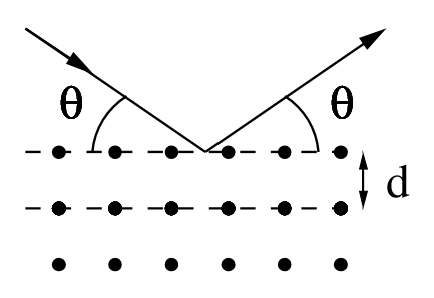
\includegraphics[width=6cm]{Bilder/Bragg.png}
    \caption{Hier ist ein Schema der Bragg'schen Reflektion aufgeführt.}
    \label{fig:Bragg}
\end{figure}

Nur bei einem bestimmten Glanzwinkel $\theta$ erfolgt konstruktive Interfetenz.
Der Zusammenhang zwischen Winkel und Wellenlänge beträgt
\begin{equation}
    \lambda=2 \frac{d}{n} \sin{\theta} \qquad .
    \label{eqn:Winkel}
\end{equation}



\cite{V602}
